%%%%%%%%%%%%%%%%%%%%%%%%%%%%%%%%%%%%%%%%%
% Journal Article
% LaTeX Template
% Version 1.3 (9/9/13)
%
% This template has been downloaded from:
% http://www.LaTeXTemplates.com
%
% Original author:
% Frits Wenneker (http://www.howtotex.com)
%
% License:
% CC BY-NC-SA 3.0 (http://creativecommons.org/licenses/by-nc-sa/3.0/)
%
%%%%%%%%%%%%%%%%%%%%%%%%%%%%%%%%%%%%%%%%%

%----------------------------------------------------------------------------------------
%    PACKAGES AND OTHER DOCUMENT CONFIGURATIONS
%----------------------------------------------------------------------------------------

\documentclass[twoside]{article}

\usepackage{lipsum}
\usepackage{graphicx}

\usepackage{listings}
\usepackage{color}

\lstset{
    language=Java,                % choose the language of the code
    basicstyle=\footnotesize,       % the size of the fonts that are used for the code
    numbers=left,                   % where to put the line-numbers
    numberstyle=\footnotesize,      % the size of the fonts that are used for the line-numbers
    stepnumber=1,                   % the step between two line-numbers. If it is 1 each line will be numbered
    numbersep=5pt,                  % how far the line-numbers are from the code
    backgroundcolor=\color{white},  % choose the background color. You must add \usepackage{color}
    showspaces=false,               % show spaces adding particular underscores
    showstringspaces=false,         % underline spaces within strings
    showtabs=false,                 % show tabs within strings adding particular underscores
    frame=single,           % adds a frame around the code
    tabsize=2,          % sets default tabsize to 2 spaces
    captionpos=b,           % sets the caption-position to bottom
    breaklines=true,        % sets automatic line breaking
    breakatwhitespace=false,    % sets if automatic breaks should only happen at whitespace
    escapeinside={\%*}{*)}          % if you want to add a comment within your code
}

\usepackage{courier}
\usepackage[sc]{mathpazo} % Use the Palatino font
\usepackage[T1]{fontenc} % Use 8-bit encoding that has 256 glyphs
\linespread{1.05} % Line spacing - Palatino needs more space between lines
\usepackage{microtype} % Slightly tweak font spacing for aesthetics

\usepackage[hmarginratio=1:1,top=32mm,columnsep=20pt]{geometry} % Document margins
\usepackage{multicol} % Used for the two-column layout of the document
\usepackage[hang, small,labelfont=bf,up,textfont=it,up]{caption} % Custom captions under/above floats in tables or figures
\usepackage{booktabs} % Horizontal rules in tables
\usepackage{float} % Required for tables and figures in the multi-column environment - they need to be placed in specific locations with the [H] (e.g. \begin{table}[H])
\usepackage{hyperref} % For hyperlinks in the PDF

\usepackage{lettrine} % The lettrine is the first enlarged letter at the beginning of the text
\usepackage{paralist} % Used for the compactitem environment which makes bullet points with less space between them

\usepackage{abstract} % Allows abstract customization
\renewcommand{\abstractnamefont}{\normalfont\bfseries} % Set the "Abstract" text to bold
\renewcommand{\abstracttextfont}{\normalfont\small\itshape} % Set the abstract itself to small italic text

\usepackage{titlesec} % Allows customization of titles
\renewcommand\thesection{\Roman{section}} % Roman numerals for the sections
\renewcommand\thesubsection{\Roman{subsection}} % Roman numerals for subsections
\titleformat{\section}[block]{\large\scshape}{\thesection.}{1em}{} % Change the look of the section titles
\titleformat{\subsection}[block]{\large}{\thesubsection.}{1em}{} % Change the look of the section titles

\usepackage{fancyhdr} % Headers and footers
\pagestyle{fancy} % All pages have headers and footers
\fancyhead{} % Blank out the default header
\fancyfoot{} % Blank out the default footer
\fancyhead[C]{Design Milestone $\bullet$ 6.005 Project 2 $\bullet$ 2013 Dec 3} % Custom header text
\fancyfoot[RO,LE]{\thepage} % Custom footer text

%----------------------------------------------------------------------------------------
%    TITLE SECTION
%----------------------------------------------------------------------------------------

\title{\vspace{-15mm}\fontsize{24pt}{10pt}\selectfont\textbf{Design Milestone}} % Article title

\author{
\large
\textsc{Andre Aboulian, Cathleen Gendron, \& Jon Beaulieu}\\[2mm] % member name
\normalsize 6.005 Software Construction - Fall 2013 - Project 2: "Collaborative Whiteboard"
\vspace{-5mm}
}
\date{}

%----------------------------------------------------------------------------------------

\begin{document}

\maketitle % Insert title

\thispagestyle{fancy} % All pages have headers and footers

\hspace{10mm}

\section{User Functionality Abstract}

\subsection{Components}

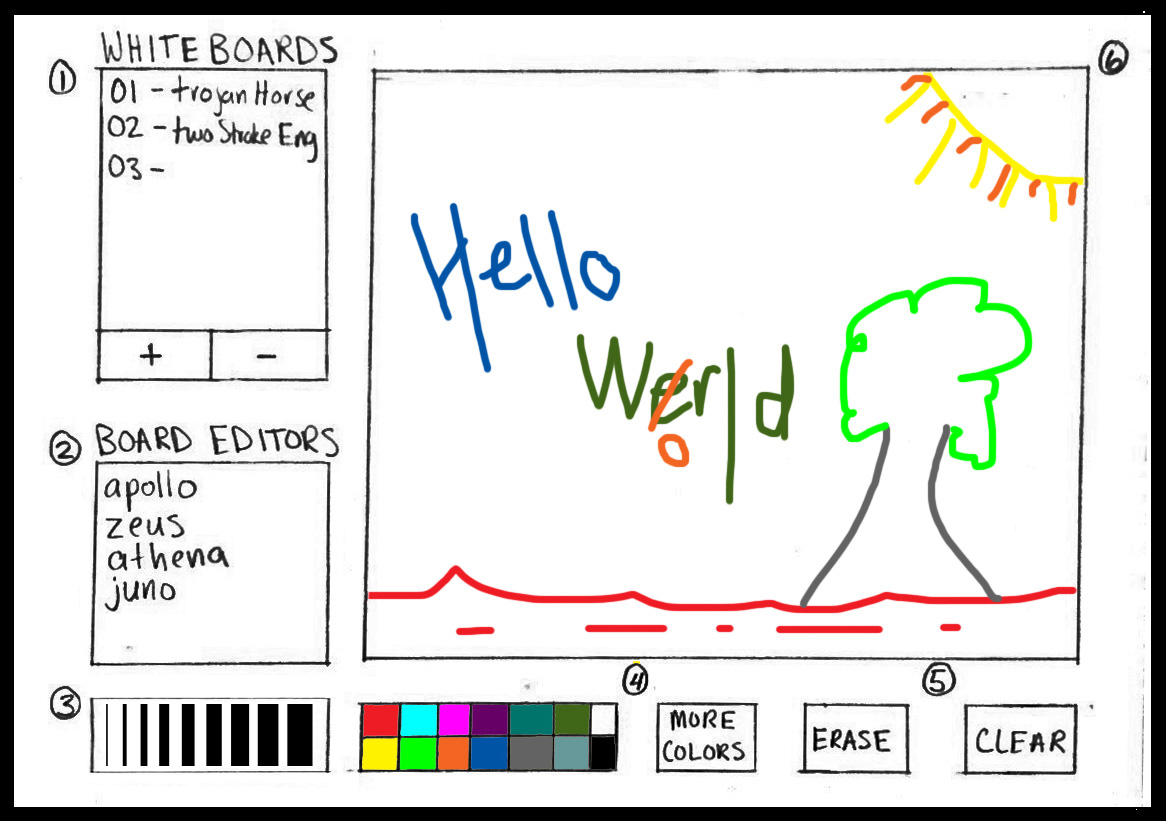
\includegraphics[keepaspectratio=1,width=6in]{img/gui-sketch.jpg}

\subsubsection{Selector}

The board selector in the left pane includes a list of all current whiteboards and appears the same for all users. Each line represents an individual board, which are numbered sequentially and named by the user. Upon clicking the "+" button, the user will be prompted to name the new board. When the board has been created on the server, it will be appended to the list for each user. Selecting a board in the list will download the board from the server, overwrite the local copy if one exists, and display the board in the canvas window. 

\subsubsection{Board Editors}

Displays a list of users, including the viewer, who are currently modifying the selected board. This list will be updated as users enter and exit the board.

\subsubsection{Thickness Selector}

This tool allows the user to select a brush/eraser thickness for drawing on the whiteboard.

\subsubsection{Color Selector}

The main color palette displays a grid of colors from which the user can choose to paint with. The color currently in use will be highlighted. Clicking the "more colors" button will open Swing's built-in color chooser, which will offer a larger selection of colors.

\subsubsection{Erasing Tools}

The erase button will allow the user to toggle between erasing and painting. "Erasing" will be defined as drawing with a white selection. Erasing will happen in the same order as drawing, so whichever request reaches the server first will erase all that has been drawn under it. Toggling back to painting will restore the user's previous color choice.

\subsubsection{Whiteboard Window}

Displays the currently selected whiteboard, including all of its drawn strokes and erasures. The whiteboard be real-time interactive to allow users to collaborate simultaneously. Edits will be made in the order that modifications reach the server. In other words, a stroke logged on the server at a specific instant will be drawn over any strokes drawn before that instant.

\subsection{Behavior}

\paragraph{Erasing}

Because the default canvas color is white, erasing will function the same as drawing with the color white selected.  The thickness functionality that is present during normal drawing will continue to work with erasing. The Erase button on the client GUI will function as a toggle. Clicking the button once will switch to erasing mode, which essentially is simply switching the client's selected color to white. At this time, the user's previously selected color will be stored for future use. Clicking the button a second time will return the user's selected color to what is was before the user entered erasing mode.

\paragraph{Editing a Deleted Board}

Clients should not be allowed to edit a board that has been deleted by another user. To prevent this, users who are working on a board when it is marked for deletion by another user will be presented with a message box, stating that their board has been deleted.  The deleted board then becomes unselected by any client GUIs who had the board selected at the time of deletion, forcing users to select a different whiteboard to work on. Simultaneously, the board will be removed from the master list of whiteboards available, so that no users in the future may accidentally select the deleted board.

\section{Server-Client Communication}

\subsection{Protocol}

\subsubsection{Grammar}
The following grammar will facilitate the text-based communication between the clients and the server. The server will send \texttt{StoC\_MSG} messages to the client, which will be able to send \texttt{CtoS\_MSG} messages back to the server.

\vspace{5mm}

\setlength{\parindent}{0in}

\texttt{StoC\_MSG :== (STROKE | BRD\_INFO | BRD\_DEL | USER\_INIT | BRD\_USERS) N}\\

\texttt{CtoS\_MSG :== (STROKE | SEL | BRD\_REQ | BRD\_DEL | BRD\_ALL | USER\_REQ) N}\\


\texttt{STROKE :== "stroke" S BOARD\_ID S THICK S COORDS S COLOR}\\
\texttt{COORDS :== X1 S Y1 S X2 S Y2}\\
\texttt{X1, Y1, X2, Y2 :== INT}\\
\texttt{COLOR :== [0-255] S [0-255] S [0-255]}\\
\texttt{THICK :== [1-10]}\\

\texttt{SEL :== "select" S BOARD\_ID}\\

\texttt{BRD\_REQ :== "board\_req" S NAME}\\
\texttt{BRD\_ALL :== "board\_all"}\\
\texttt{BRD\_INFO :== "board" S BOARD\_ID S NAME}\\
\texttt{BRD\_DEL :== "del" S BOARD\_ID}\\
\texttt{BRD\_USERS :== "board\_users" S BOARD\_ID (S USER\_NAME)+}\\

\texttt{USER\_REQ :== "user\_req" S USER\_NAME}\\
\texttt{USER\_INIT :== "you\_are" S USER\_NAME}\\

\texttt{NAME :== [$\char`\^$N]}\\
\texttt{USER\_NAME :== [A-Za-z]([A-Za-z0-9]?)+}\\
\texttt{BOARD\_ID :== INT}\\

\texttt{INT :== [0-9]+}\\
\texttt{N :== "$\backslash$r?$\backslash$n"}\\
\texttt{S :== " "}\\

\setlength{\parindent}{15pt} %default

\subsubsection{Definitions and Usage}
Below is the definition for each of the messages that can be sent across the network. Note that particular messages warrant a response after processing, and those returned messages are included in the definition.

\paragraph{\texttt{STROKE}} A \texttt{STROKE} message is sent from a client to the server upon drawing a line.
\begin{enumerate}
\item A \texttt{WhiteLine} object is created for the line from (\texttt{X1},\texttt{Y1}) to (\texttt{X2},\texttt{Y2}) with thickness \texttt{THICK} and color \texttt{COLOR}. It is then added to the \texttt{MasterBoard} corresponding to the provided \texttt{BOARD\_ID}.
\item The \texttt{STROKE} message is forwarded to all clients who are currently editing the same board, so that the line can be incorporated onto their whiteboards.
\end{enumerate}

\paragraph{\texttt{SEL}} Upon selecting a different board, the client sends a \texttt{SEL} request to the server.
\begin{enumerate}
\item The server clears all stroke messages queued to update the client's whiteboard.
\item The server disassociates the client with the current whiteboard if one is assigned and associates the client with the requested board.
\item A \texttt{BRD\_USERS} message is sent to all users of the requested board, with the addition of the new editor, to inform them of the change. Another \texttt{BRD\_USERS} message is sent to all users of the previous board, with the omission of the removed editor, to inform them of the change.
\item A sequence of \texttt{STROKE} messages are sent to the client to recreate the current state of the selected whiteboard.
\end{enumerate}

\paragraph{\texttt{BRD\_REQ}} When the client wants to create a new board, it send a \texttt{BRD\_REQ} message with a properly formatted \texttt{NAME}.
\begin{enumerate}
\item The server initializes a new \texttt{MasterBoard} object with relevant properties and adds it to its list of boards.
\item A \texttt{BRD\_INFO} message for the new board is sent to all connected clients to inform them of the newly available whiteboard. The clients add this board to their list of available boards.
\end{enumerate}

\paragraph{\texttt{BRD\_ALL}} This is often called by the client upon initialization. It prompts a series of \texttt{BRD\_INFO} replies for all existing boards.

\paragraph{\texttt{BRD\_DEL}} When the client wants to remove a board, it send a \texttt{BRD\_DEL} message to the server.
\begin{enumerate}
\item If the provided \texttt{BOARD\_ID} exists, the server removes the designated board from its central list of boards.
\item The \texttt{BRD\_DEL} message is forwarded to all clients to signify that the board is no longer available. The clients remove this board from their list of available boards.
\end{enumerate}

\paragraph{\texttt{USER\_REQ}} Upon entering a username in the client application, a \texttt{USER\_REQ} message with a properly formatted \texttt{USER\_NAME} will be sent to the server to request the desired username.
\begin{enumerate}
\item The requested username is checked against existing username. If the name already exists, a name is generated using the new board's ID number.
\item A \texttt{User} object with relevant properties is created to represent the new client.
\item A \texttt{USER\_INIT} message is sent to the client to inform it of its acquired username.
\end{enumerate}

Note that \texttt{BRD\_USERS}, \texttt{BRD\_INFO}, and \texttt{USER\_INIT} are used solely as replies and are included in the descriptions above.


\subsection{Data Transport}
For a detailed explanation of the communication method between the clients and the server, please see the "Threads and Queues" section.

\section{Data Type}

\subsection{\texttt{MasterBoard}}

\subsubsection{Description}
\texttt{MasterBoard} represents a single whiteboard on the server. The instance is held by several \texttt{User} objects editing the board, which are mutually stored in the \texttt{MasterBoard} object; in other words, the board is aware of its editors and the editors are aware of the board.

\subsubsection{Fields}
\begin{itemize}
\item \texttt{final String name} - The name of the board in the grammar format \texttt{NAME}.
\item \texttt{final int id\_num} - The unique identification number of the board.
\item \texttt{static final AtomicInteger nextID} - The identification number of the successive board to be created.
\item \texttt{final static int Y\_SIZE, X\_SIZE} - The X and Y dimensions of the whiteboard.
\item \texttt{final ArrayList<WhiteLine> strokes} - A list of the strokes drawn on the whiteboard. The ordering of these strokes corresponds to the sequence in which modifications were made on the server and the layering of the segments.
\item \texttt{final ArrayList<User> users} - A list of editors currently modifying the board.
\end{itemize}

\subsubsection{Methods}
\begin{itemize}
%\item \texttt{WhiteLine[] allStrokes()} - Returns all the strokes that have been made on the board thus far by locking on \texttt{strokes} list.
\item \texttt{void makeStroke(WhiteLine stroke)} - Adds the new \texttt{stroke} while locking on the \texttt{strokes} list. Proceeds to call \texttt{incorporateStroke()} on each user while locking on the \texttt{users} list.
\item \texttt{void clearBoard()} - Clears all strokes from the board while locking on the \texttt{strokes} list. Proceeds to call \texttt{notifyClear()} on each user while locking on the \texttt{users} list.
\item \texttt{void addUser(User user)} - Adds the new \texttt{user} while locking on the \texttt{users} list. Then proceeds to send all existing strokes to the new \texttt{user}.
\item \texttt{void removeUser(User user)} - Removes the user \texttt{user} while locking on the \texttt{users} list.
\item \texttt{void removeAllUsers()} - This method is called by the \texttt{WhiteboardServer} after the board is removed from its global list of available boards but before all \texttt{users} are notified of the board's deletion. The the \texttt{users} list within the \texttt{MasterBoard} is cleared.
\item \texttt{String getUserList()} - Returns an alphabetized, space-delimited list of current editors while locking on the \texttt{users} list.
\item \texttt{String getName()} - Returns the name of the whiteboard.
\item \texttt{int getID()} - Returns the unique identification number of the board.
\item \texttt{String toString()} - Returns the properties of the board in the form of a \texttt{BOARD\_INFO} message.
\item \texttt{boolean equals(Object other)} - Compares boards for equality on the basis of ID number.
\item \texttt{int hashCode()} - Returns the identification number of board added to $2^{25}$.
\end{itemize}

\subsubsection{In Action}
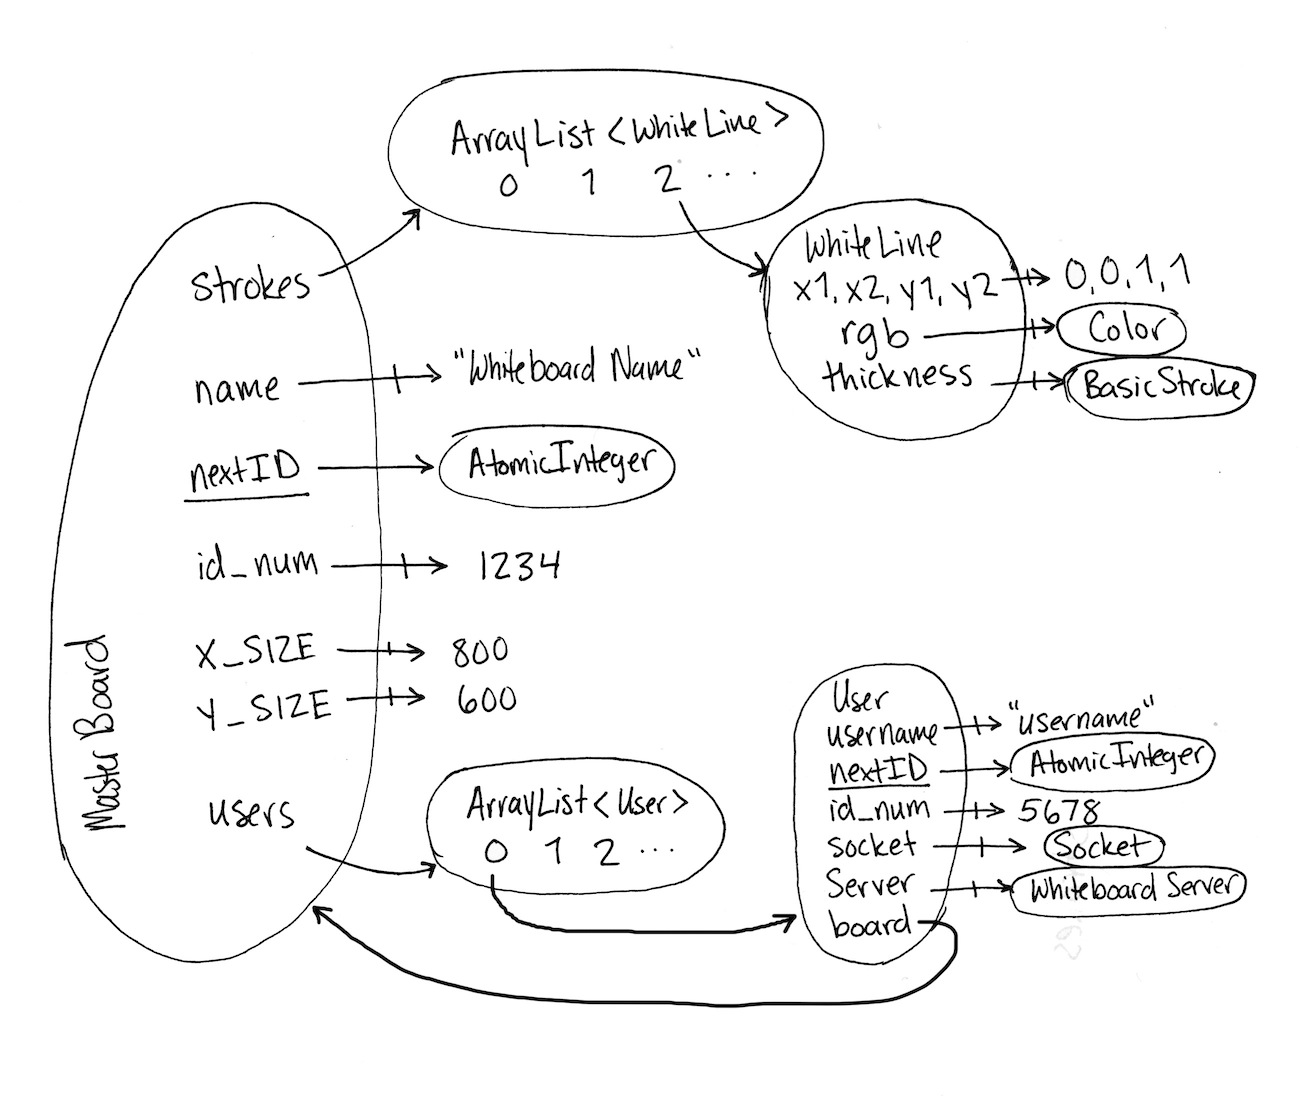
\includegraphics[keepaspectratio=1,width=6in]{img/wb-snapshot.jpg}


\subsection{\texttt{User}}

\subsubsection{Description}
Each instance of \texttt{User} represents a separate client connected to the server. \texttt{User} is not only responsible for storing properties that pertain to the client; it also facilitates the socket communication and request handling for each client.

\subsubsection{Fields}
\begin{itemize}
\item \texttt{final WhiteboardServer server} - The main server instance is stored for later global calls.
\item \texttt{MasterBoard board} - The current board being edited by the user. A null value indicates that no board is selected.
\item \texttt{final String username} - The unique acquired username assigned by the server after a username request has been made.
\item \texttt{final int id\_num} - The unique identification number of the user.
\item \texttt{static final AtomicInteger nextID} - The identification number of the successive user to be created.
\item \texttt{final Socket socket} - The socket corresponding to the client application represented by the \texttt{User} instance. The input and output streams are contained within.
\item \texttt{BlockingQueue queue} - The queue containing all outgoing messages to the connected client.
\end{itemize}

\subsubsection{Methods}
\begin{itemize}
\item \texttt{void notifyBoard(MasterBoard board)} - Queues a \texttt{BRD\_INFO} message to be sent to the client with priority. This method is called by the main \texttt{WhiteboardServer} on all \texttt{User} instances once the request for a new board has been processed.
\item \texttt{void forgetBoard(MasterBoard board)} - Queues a \texttt{BRD\_DEL} message to be sent to the client with priority. This method is called by the main \texttt{WhiteboardServer} on all \texttt{User} instances once the request to remove a whiteboard has been processed.
\item \texttt{void notifyStroke(WhiteLine stroke)} - Queues a \texttt{STROKE} message to inform the client of a new stroke drawn on the current board.
\item \texttt{void notifyClear()} - Queues a \texttt{BRD\_CLR} message to inform the client that the current board has been cleared.
\texttt{void notifyEditors(String editorList)} - Queues a \texttt{BRD\_USERS} message to inform the client of a change in editors on the current board.
\item \texttt{void handleRequest()} - Runs in a background thread and takes care of all incoming requests from the client. Appropriate actions are taken for each request, either with the \texttt{server} or on the \texttt{board}.
\item \texttt{void selectBoard(int boardID)} - This method is called upon receiving a \texttt{SEL} command from the client. The user removes itself from the current board by calling \texttt{removeUser(this)} on the locked \texttt{board}, replacing \texttt{board} with on acquired from \texttt{server.getBoard(boardID)} and calling \texttt{addUser(this)} on the new reference. All queued \texttt{STROKE} are removed since they pertain to the old board. By having called \texttt{addUser(this)}, all previously drawn strokes for the new board are queued to be sent to the client.
\item \texttt{String getName()} - Returns the username of the connected client.
\item \texttt{int getID()} - Returns the unique identification number of the connected client.
\item \texttt{int compareTo(Object other)} - Compares users for ordering on the basis of usernames.
\item \texttt{boolean equals(Object other)} - Compares users for equality on the basis of identification numbers.
\item \texttt{int hashCode()} - Returns the identification number of the user added to $2^{26}$.
\item \texttt{String toString()} - Returns the uername and ID number of the user in string format.
\end{itemize}


\subsection{\texttt{WhiteLine}}

\subsubsection{Description}
\texttt{WhiteLine} is a simple class designed to represent a drawn stroke on a whiteboard. It is used by the \texttt{MasterBoard} class on the server side and the \texttt{ClientView} class on the client side. Due to the frequent need to work with lines and the neatness of working with a single object containing the multiple properties of the line -- location, color, thickness -- we decided to have a dedicated class. The class is immutable, as all its properties are themselves immutable and stored upon construction.

\subsubsection{Fields}
\begin{itemize}
\item \texttt{final int x1, y1, x2, y2} - The coordinates of the line, which spans from \texttt{(x1,y1)} to \texttt{(x2,y2)}.
\item \texttt{final java.awt.Color color} - The color of the line. The \texttt{Color} object allows greater versatility over storing individual RGB values, as Java provides multiple methods for specifying colors. This is especially useful for using a \texttt{JColorChooser}.
\item \texttt{final java.awt.BasicStroke thickness} - The thickness of the line will be specified as a number within the range [1,10]. Numbers from this qualitative scale will be mapped to floating-point thicknesses and a \texttt{BasicStroke} object will be constructed internally.
\end{itemize}

\subsubsection{Methods}
\begin{itemize}
\item \texttt{int getX1()} - Returns the X-coordinate of the origin of the line.
\item \texttt{int getY1()} - Returns the Y-coordinate of the origin of the line.
\item \texttt{int getX2()} - Returns the X-coordinate of the terminus of the line.
\item \texttt{int getY2()} - Returns the Y-coordinate of the terminus of the line.
\item \texttt{java.awt.Color getColor()} - Returns the \texttt{Color} object corresponding to the line.
\item \texttt{java.awt.BasicStroke getThickness()} - Returns the \texttt{BasicStroke} object corresponding to the thickness value specified upon construction.
\item \texttt{String toString()} - Returns the properties of the stroke in the form of a \texttt{STROKE} message with the \texttt{BOARD\_ID} omitted.
\end{itemize}

%\texttt{String toString()}, \texttt{boolean equals()}, and \texttt{int hashCode()} have been implemented for debugging; they behave as expected.


\subsection{\texttt{ClientBoard}}

\subsubsection{Description}
\texttt{ClientBoard} is used by the client application to store basic properties about the active whiteboards, which include those created by the client and other users. A new instance is created each time the client receives a \texttt{BRD\_INFO} message. The class is immutable, as the contained properties are never changed after initialization on the server side.

\subsubsection{Fields}
\begin{itemize}
\item \texttt{final String name} - The user-assigned name of the board.
\item \texttt{final int id\_num} - The identification number assigned to the whiteboard. This number is assigned by the server in the order that whiteboards are created; it cannot be the same for any two boards.
\end{itemize}

\subsubsection{Methods}
\begin{itemize}
\item \texttt{String getName()} - Returns the name of the board.
\item \texttt{int getID()} - Returns the identification number of the board.
\item \texttt{int compareTo(Object other)} - Compares two boards on the basis of their ID numbers. Overrides the default comparison method and follows its conventions.
\item \texttt{String toString()} - Returns the properties of the board in the form of a \texttt{BOARD\_INFO} message.
\end{itemize}


\subsection{\texttt{ClientView extends JPanel}}

\subsubsection{Description}
\texttt{ClientView} has the simple task of managing the drawing canvas of the current board. It fulfills the role of the "View" component of the Model-View-Controller structure. Since the class that extends \texttt{JPanel}, it is used directly as a component within the client application.

\subsubsection{Fields}
\begin{itemize}
\item \texttt{final Image buffer} - The buffer where changes are made before being drawn to the displayed canvas.
\item \texttt{final static int Y\_SIZE, X\_SIZE} - The X and Y dimensions of the whiteboard.
\end{itemize}

\subsubsection{Methods}
\begin{itemize}
\item \texttt{void drawLine(WhiteLine line)} - Draws the designated \texttt{line} on the \texttt{buffer}, which does not appear on the displayed canvas.
\item \texttt{void clear()} - Clears the displayed canvas and the contents of the \texttt{buffer} immediately.
\item \texttt{void push()} - Displays all changes that were made since the last time \texttt{push()} or \texttt{clear()} was called. Copies the contents of the \texttt{buffer} to the displayed canvas.
\end{itemize}

\newpage
\subsection{Board Switching}
The following sequence of steps defines the back-end operation of changing a client's whiteboard.
\begin{enumerate}
\item The \texttt{User} instance that represents a specific connected client begins with a reference to a \texttt{MasterBoard} instance. That \texttt{MasterBoard} instance has that associated \texttt{User} in its \texttt{users} list. The client then selects another board in the list of available boards, sending a \texttt{SEL} message to the server and is processed in the \texttt{User} class. \\  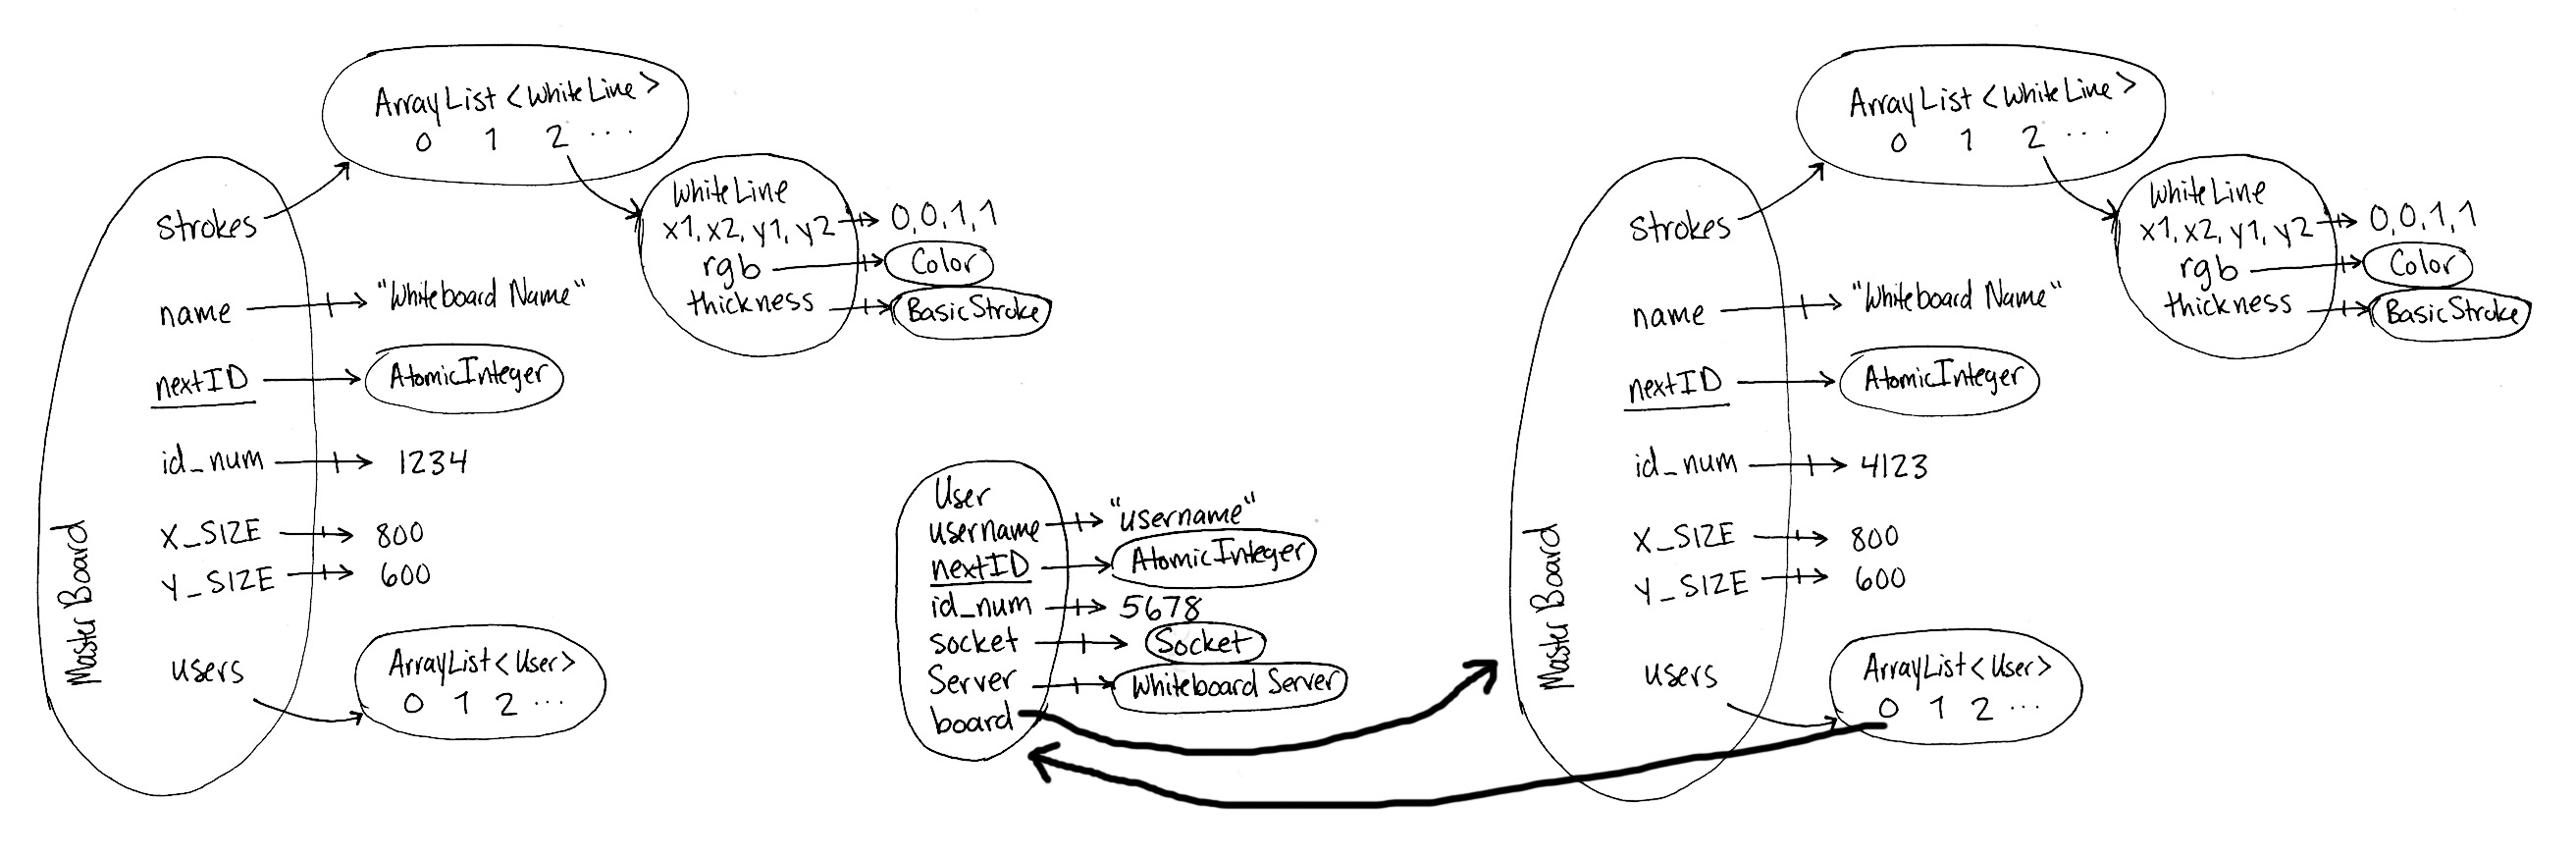
\includegraphics[keepaspectratio=1,width=6in]{img/switch-sequence/switch-00.jpg}
\item The \texttt{User} calls \texttt{board.removeUser(this)} on its current board, causing the board to no longer identify the client as one of its users. \\ 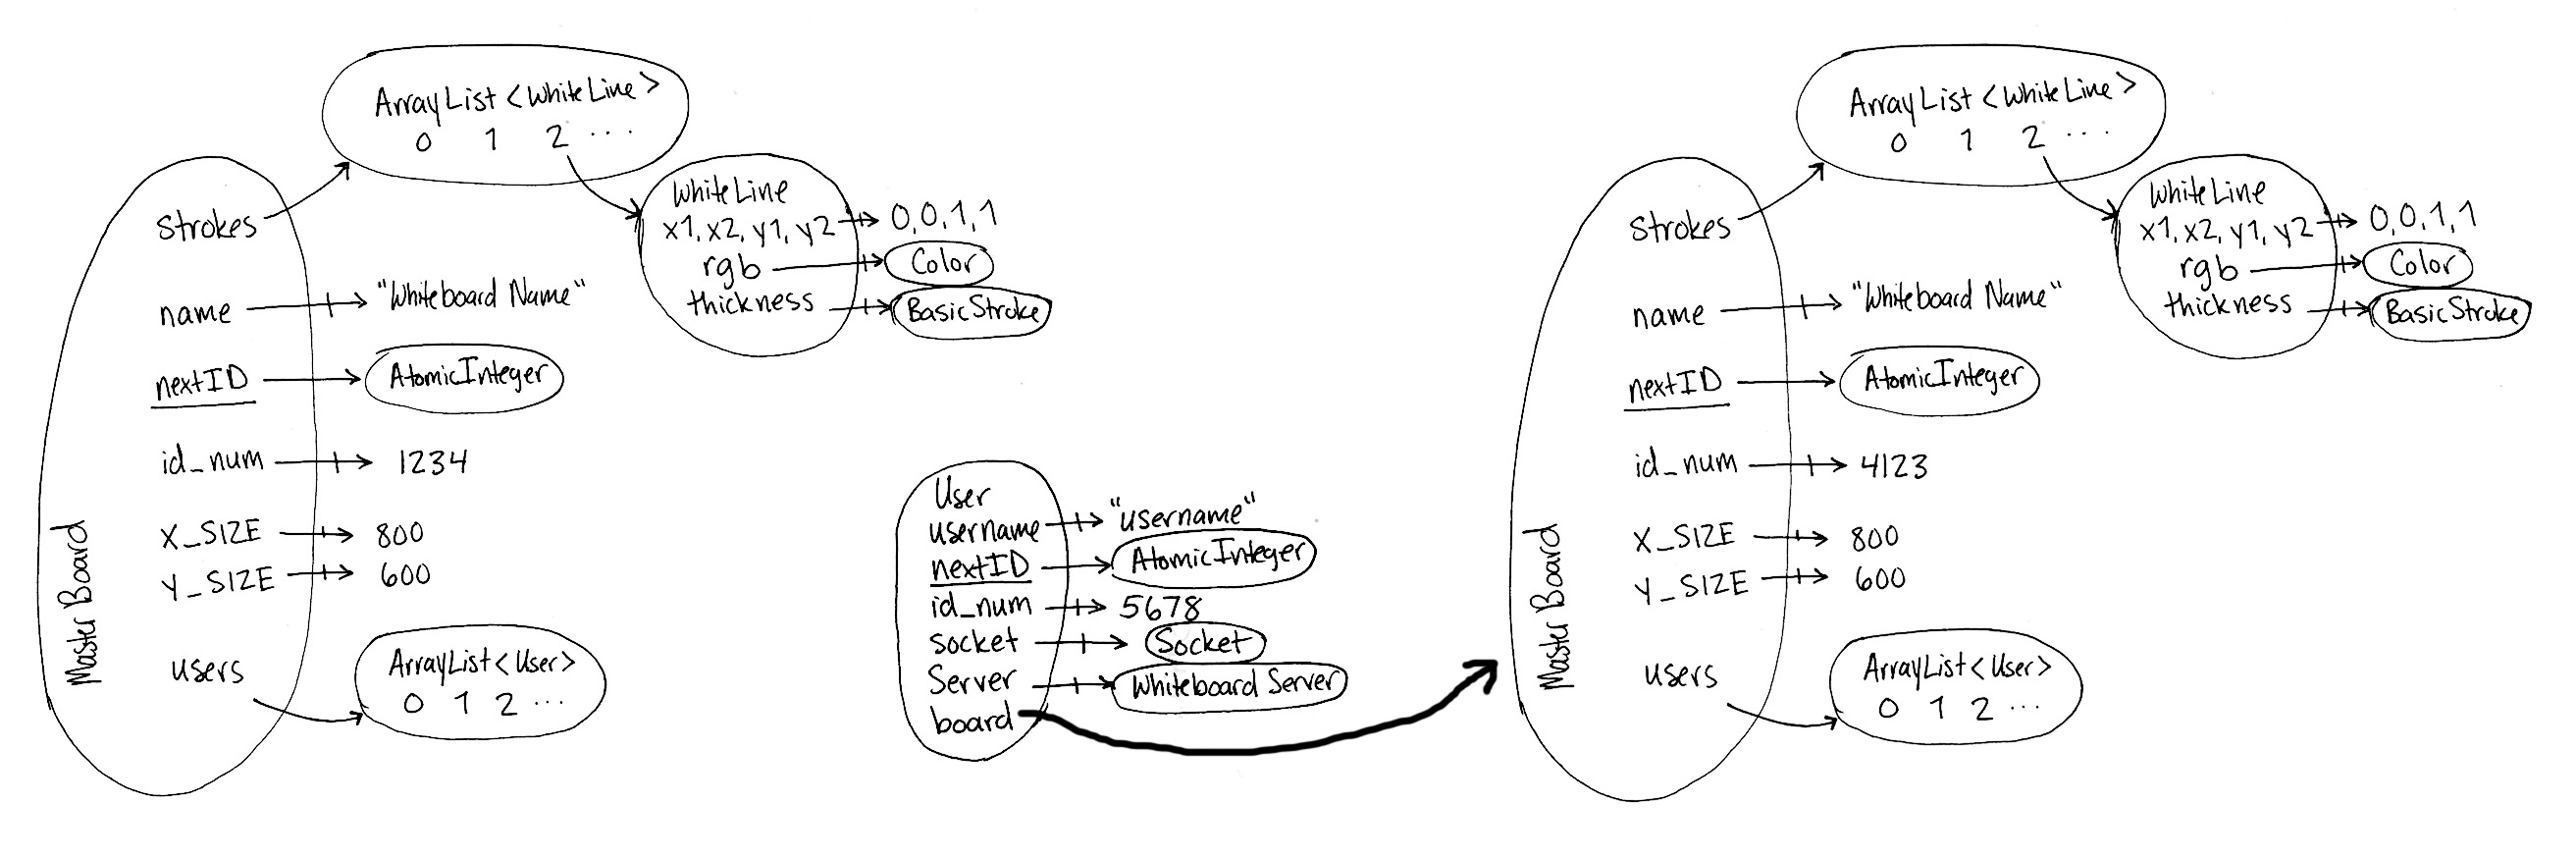
\includegraphics[keepaspectratio=1,width=6in]{img/switch-sequence/switch-01.jpg}
\item The \texttt{User} executes \texttt{board = server.getBoard(id\_num)} obtain the requested board from the server and reassign its reference to it. \\ 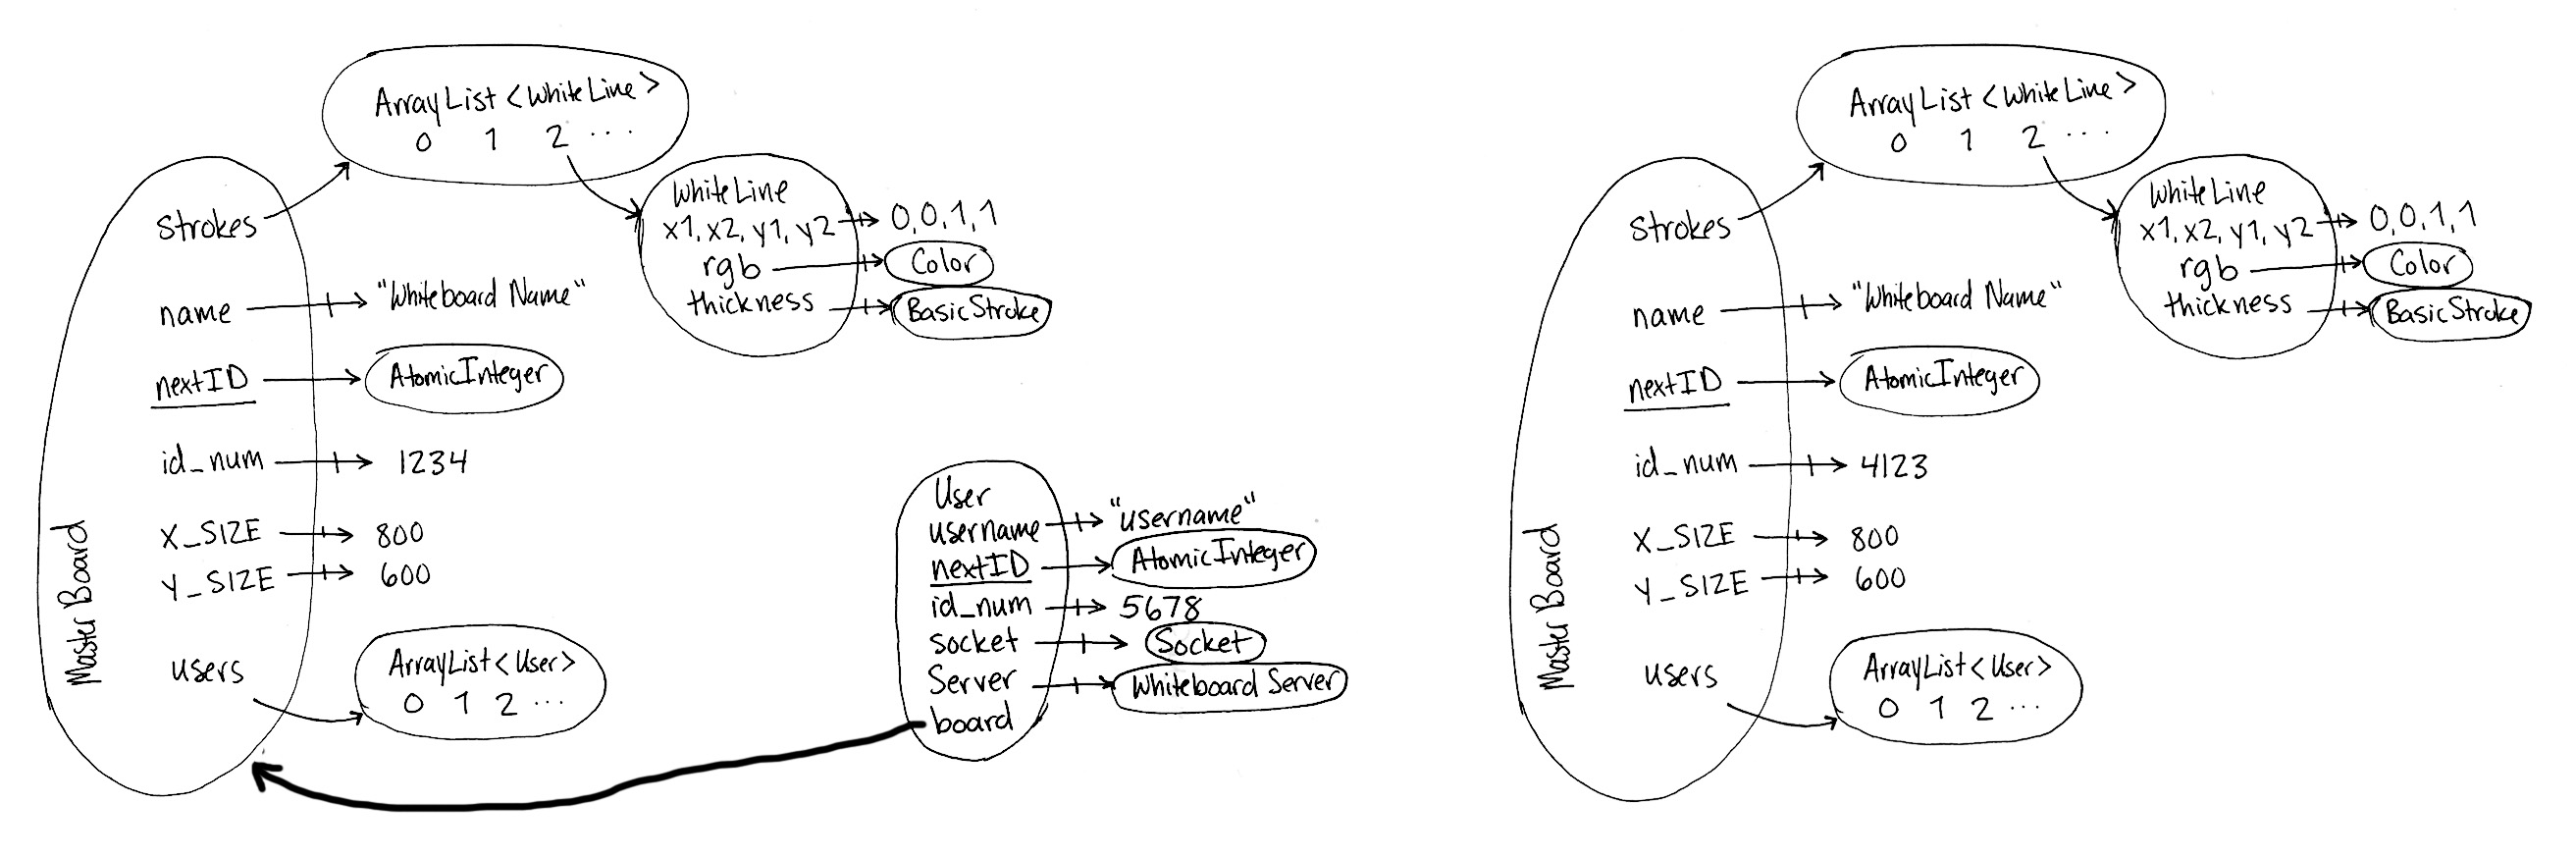
\includegraphics[keepaspectratio=1,width=6in]{img/switch-sequence/switch-02.jpg}
\item The \texttt{User} calls \texttt{board.addUser(this)} on its new board, causing the board to identify the client as one of its users. \\ 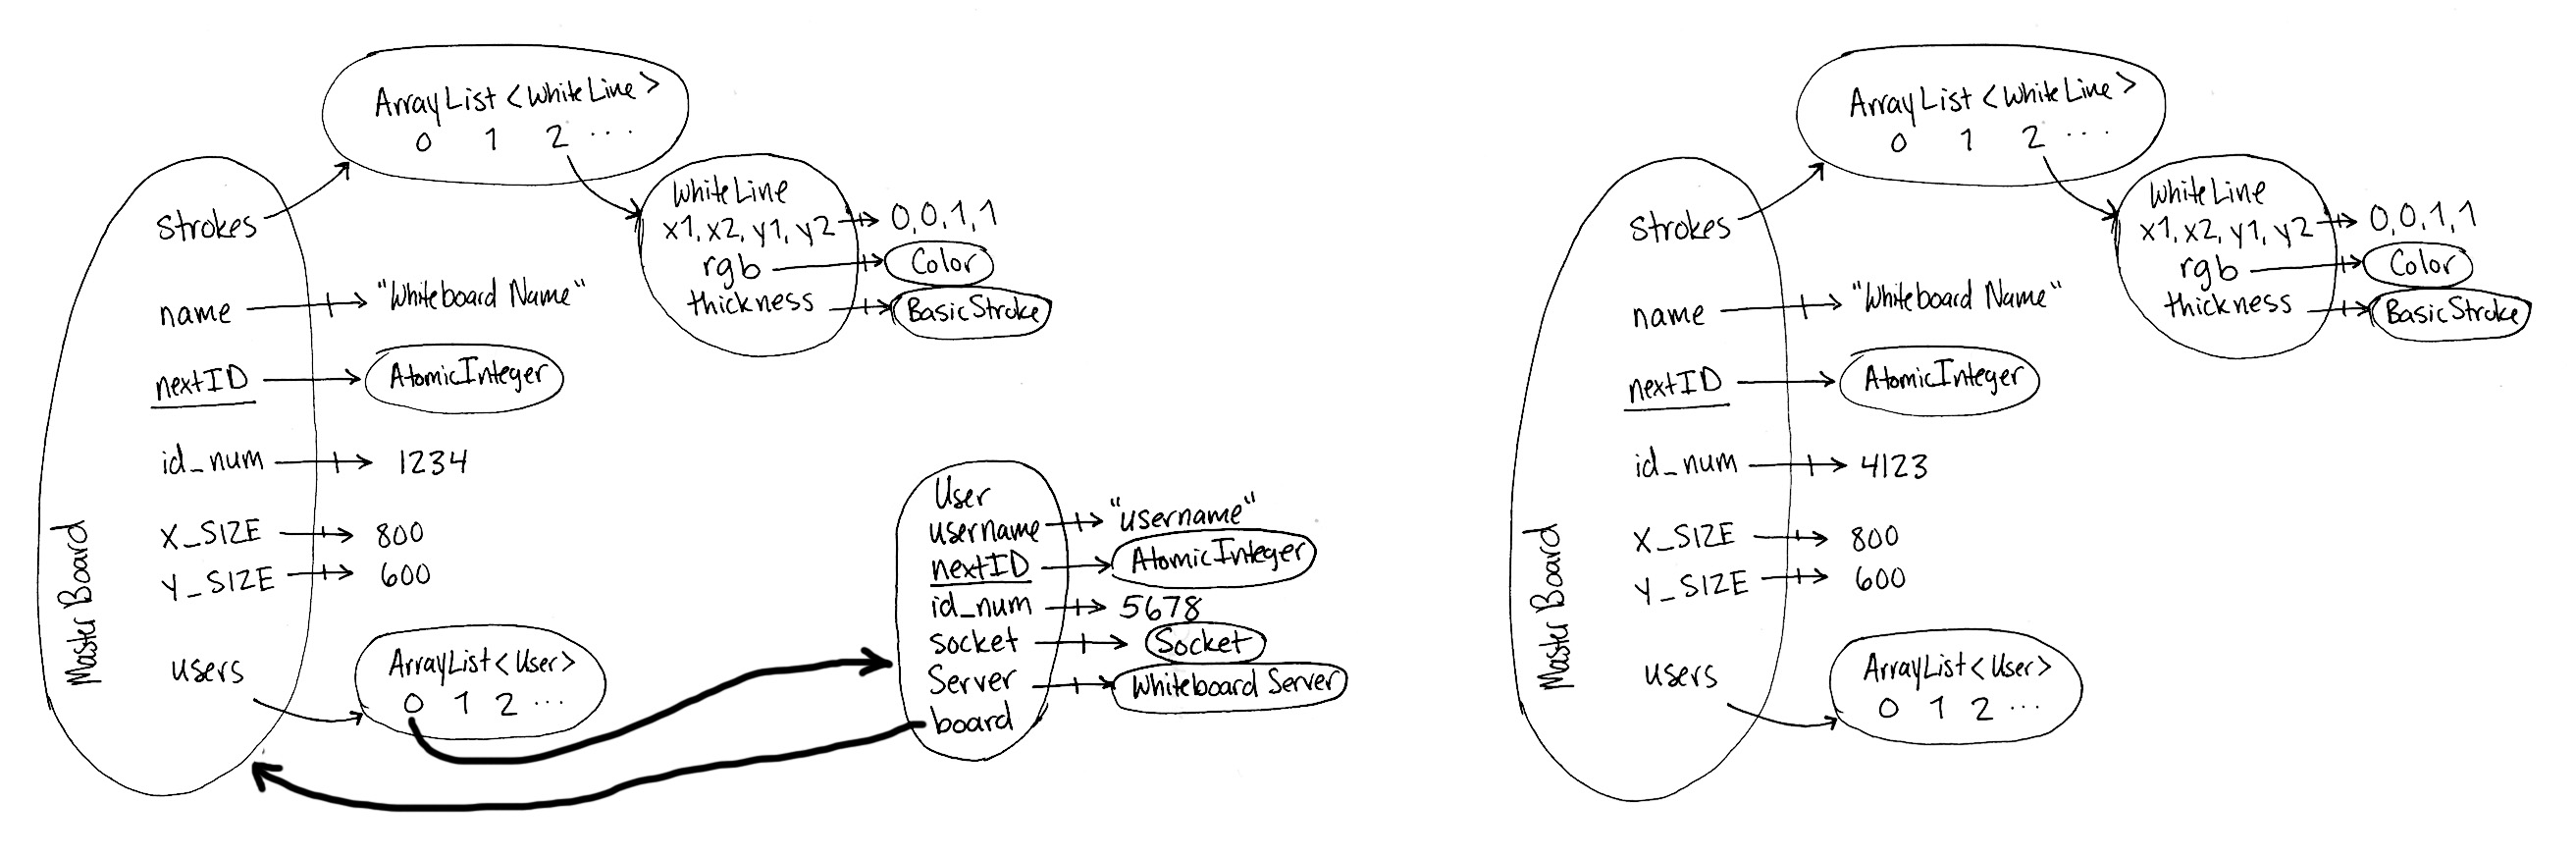
\includegraphics[keepaspectratio=1,width=6in]{img/switch-sequence/switch-03.jpg}
\end{enumerate}



%WhiteboardServer and WhiteboardClient specified here

\section{Threads and Queues}

\paragraph{Client} The GUI maintains one \texttt{SwingWorker} thread, which reads and processes requests received from the server. Possible messages include notifications of a new Whiteboard, a deleted Whiteboard, or a new Stroke. Note that output is written directly in the client application in the main thread.

\paragraph{User} Each \texttt{User} object on the server object holds a socket connected to an individual client. The \texttt{User} class has two outgoing message queues: one is dedicated to \texttt{STROKE} messages, whereas the other sends general messages. The outgoing stroke queue can be cleared upon changing boards without affecting other messages that need to be sent to the client. The \texttt{User} maintains two threads, one which receives and handles requests from the client, and another which sends messages to the client. The latter thread consumes from both the message queue and the stroke queue, prioritizing sending general messages over stroke updates.

\paragraph{MasterBoard} Each time a stroke is written to a \texttt{MasterBoard}, the \texttt{WhiteLine} passed is queued for later processing. Each \texttt{MasterBoard} has one thread which consumes lines from this queue, makes the change, and sends the update to all users.

\paragraph{WhiteboardServer} The \texttt{WhiteboardServer} has a thread continuously running to accepts new users that connect to its server-side socket. Each time a user connects, the corresponding \texttt{Socket} instance is passed to a new dedicated thread wile the original thread continues to accept new users. In these individual threads, the username handshake is resolved and a new \texttt{User} instance is created. In other words, there is one thread always running and there are as many additional threads as there are clients being instantiated. Each additional thread is closed once the user has been created.

\section{Thread Safety}

\subsection{Processes}

\subsubsection{Adding New Users}

Upon receiving a \texttt{USER\_REQ} message, the WhiteboardServer calls \texttt{createNewUser} on the main server thread. This instantiates the new User object and adds it to the \texttt{users} ArrayList. This method locks on the \texttt{boards} field first, and then the \texttt{users} field. This ensures that only one User is created at a time, and that behavior that is dependent other User objects, such as username and ID assignment, is consistent.

\subsubsection{Adding and Removing Boards}

Upon receiving a \texttt{BRD\_REQ} message, the WhiteboardServer calls \texttt{createBoard}, which instantiates the new MasterBoard object and adds it to the \texttt{boards} ArrayList. This method locks on the \texttt{boards} field first, and then the \texttt{users} field. If multiple requests for a new board are sent, the locks ensure that another board is not created until the current board is created, added to the ArrayList, and all Users are updated with these changes.

Upon receiving a \texttt{BRD\_DEL} message, the WhiteboardServer calls \texttt{removeBoard}. This removes the board from the server's \texttt{boards} ArrayList, as well disassociating all Users currently active on that board. This method locks on the \texttt{boards} field and then the \texttt{users}, so that only one board can be deleted at a time, and so that one thread cannot be deleting a board from the ArrayList while another is attempting to add one.

\subsubsection{Drawing Strokes}

Each time a line is drawn on a client's Canvas, a request is sent from the WhiteboardClient to the MasterBoard via a buffer. The MasterBoard puts this message on a queue of pending requests, then locks on the \texttt{strokes} ArrayList and appends the stroke encoded in the message. The use of the threadsafe BlockingQueue ensures that all strokes are sent from the GUI to the MasterBoard in the correct order. Before releasing the lock, all Users associated with this board are informed of the newly added stroke.

\subsubsection{Selecting Boards}

When the client selects a new board, the server fetches the board to be sent. The User calls \texttt{allStrokes} to obtain all of the strokes associated with the new board. This method locks on the \texttt{strokes} ArrayList, so that no new strokes can be added before the User has received the entire ArrayList. The User also adds itself to the MasterBoard's \texttt{users} ArrayList, locking on that field to ensure that only one User is added at a time.

\subsection{Averted Race Conditions}

\subsubsection{New Board and New User}

Both \texttt{BRD\_REQ} and \texttt{USER\_REQ} messages are handled on the main server thread. Since only one of these requests can be processed at a time, there cannot be any racing between the two methods that would potentially cause a newly created board to be lost for some Users. 

\subsubsection{Remove Board and New User}

Similar to the strategy in the previous section, both \texttt{DEL\_BRD} and \texttt{USER\_REQ} requests are handled on the main server thread. This eliminates any racing in which a new User would be created and still receive a board that had actually been deleted.

\subsubsection{Concurrent Strokes}

Because the GUI sends the new stroke messages through a BlockingQueue, the order is preserved. The MasterBoard then appends the strokes to its \texttt{strokes} in the order that they are received from the clients. (Note that this is not necessarily exactly the same as the order in which each stroke is sent from each GUI, but every User will receive strokes in the exact same order when receiving updates from the MasterBoard.) Because the \texttt{makeStrokes} method locks on \texttt{strokes} while it processes a request, only one stroke will be processed at a time, and the risk of losing strokes or having clients receive stroke updates in different orders is eliminated. Similarly, while a newly selected board is being transferred to a client, no new strokes can be added, to eliminate these same risks.

\subsubsection{Atomic ID Generation}

All object IDs are generated by a static AtomicInteger associated with each class. Because the AtomicInteger is threadsafe, any risks associated with interleaving integer operations are eliminated.

\subsection{Thread-Safe Collections}

The server-side classes \texttt{User} and \texttt{MasterBoard} contain a number of ArrayList fields, referenced in the preceding sections. With the exception of \texttt{strokes} in \texttt{MasterBoard}, all of these fields will utilize the thread-safe synchronized wrapper, to add additional protection against concurrency problems, such as deadlock. The \texttt{strokes} field will not use this wrapper, because the \texttt{MasterBoard} uses a BlockingQueue for pending changes, which ensures that the \texttt{strokes} ArrayList is not accessed in multiple threads concurrently, and to avoid the synchronized wrapper's performance penalty on an object accessed so frequently.

\section{Testing}
Overview Text

\subsection{Constructor Testing}

\subsubsection{New Board} 

\paragraph{Valid Name}
Test the creation of a new whiteboard with a valid name. This is simple to conduct by simply clicking the “+” button under the list of whiteboards. The client should be prompted to enter a name. Enter a valid name that is not already in use. The server should create a new \texttt{MasterBoard} object and add it to the list of existing boards.  This should be seen by all clients. The new whiteboard should be completely white.

\paragraph{Invalid Name}
Test the creation of a new whiteboard with an invalid name. Again, conduct by simply clicking the “+” button under the list of whiteboards. The client should be prompted to enter a name. Enter a name that is already in use. The server should inform the user that the name is already in use, then create a new \texttt{MasterBoard} object with a default name assigned by the server. Again, this new \texttt{MasterBoard} should be added to the list of existing boards, and should be seen by all users. The new whiteboard should be completely white.

\subsubsection{New User}

\paragraph{Valid Name}
Connect to the whiteboard server.  When prompted for a username, enter a valid one – that is, one that is not already in use.  The server should accept this name and assign it to the user, then allow the user to select a board and begin drawing.

\paragraph{Invalid Name}
Connect to the whiteboard server. When prompted for a username, enter a name that is already in use. The server should notify the new client that his/her choice of username is already in use, and should assign the new user a different (valid) name from a predefined list of names.  The new client should then be allowed to select a board and begin drawing.

\subsection{Normal Functionality}

\subsubsection{Loading a Board}
Tests behavior when a user attempts to load an existing board to work on.  This will happen when a client clicks on a board name from the list of existing board on the left of the GUI.  Expected behavior: The \texttt{User} associated with this client will be removed from the list of users working on the previous board.  It will then be added to the list of users working on the newly selected board.  This will be reflected on the list of users on the bottom left of the GUI for anyone working on the newly selected board.  In addition, the client who changed selections will have his drawing space refreshed to contain an up-to-date version of his/her newly selected board.  The client will then be able to modify this board as usual.

\subsubsection{Creating a New Board}
Tests behavior when a client attempts to create a new multi-user whiteboard.  This event will occur when the client clicks the “+” button located below the list of existing whiteboards.  When this button is clicked, the client will be prompted to enter a name for the new whiteboard. If the name is not valid (already in use), the server will assign a default one.  The new whiteboard will appear in the list of existing whiteboards in the GUI, so that all users are able to access it.  The client who created the whiteboard will automatically have his GUI switched so that he is viewing the newly created board, in accordance to the “Loading a Board” test above. The newly created \texttt{MasterBoard} will begin as a blank white canvas, with the standard 800x600 pixel dimensions.

\subsubsection{Deleting a Board}
Tests behavior when a client deletes an existing board. This will occur when a client clicks the “-” button located below the list of existing whiteboards.  To prevent clients from accidentally (or purposefully) deleting others’ work, the “-” button will always delete the whiteboard that the client is currently viewing. In addition, it will be impossible to delete a whiteboard if only one is currently is existence, to prevents errors arising from a lack of whiteboards.  Deletion will completely remove the selected \texttt{MasterBoard} object from the server memory. It will be reflected in the list of whiteboards that appears in the user GUI, where the name of the deleted whiteboard will be removed for all users. Other clients who are working on a whiteboard when it is deleted will be notified via a pop-up message that their board has been deleted.  Their workspace will then not have any whiteboard selected, meaning that they will need to load another whiteboard before continuing to draw.  All requests sent to the server referencing the deleted whiteboard will be ignored after board deletion.

\subsubsection{Choosing Stroke Thickness}
This will test the user’s ability to select a stroke thickness for drawing purposes. Thickness will be controlled through the \texttt{Width} component of a \texttt{Java 2D Stroke}. A variety of stroke widths will be available for selection from the thickness panel near the bottom left corner of the GUI. Each image in this area will be associated with a specified stroke thickness. Clicking on one of these images will switch the user’s default stroke thickness to the width associated with the selected image.

\subsubsection{Choosing Stroke Color}
This will test the user’s ability to select a drawing color. Thickness will be controlled through the \texttt{Color} component of \texttt{Java 2D Graphics}. A variety of colors will be available for selection from the color panel along the bottom of the GUI. Clicking on one of these given colors will switch the user’s default stroke color to the selected color.

\subsubsection{"More Colors" Button}
In addition to choosing a color as listed above, users should be able to select from a wider range of colors in a \texttt{JColorChooser} window. This window will appear when a client clicks the “more colors” button to the right of the GUI’s color panel. The client will then be able to change his default stroke color to any color provided in the \texttt{JColorChooser} window. If the user clicks outside of the \texttt{JColorChooser} window while it is open, the window will be closed and the client’s color will not be changed.

\subsubsection{"Erase" Button}
The erase button will function as a toggle, switching the client between his previously chosen color and white. As the default board color is white, painting with white will appear visually the same as erasing an existing portion of the whiteboard. When the user selects “erase” for the first time, his/her color choice will switch to white.  Clicking the “erase” button a second time will switch the user back to whichever color was selected before “erase” was clicked the first time.

\subsubsection{"Clear" Button}
The “clear” button will completely erase the client’s currently selected board.  On the server side, this will delete all strokes that have ever been applied to the selected whiteboard. As a result, the whiteboard will appear as it did when it was first created – blank white. This change, like any other painting operation, will be seen by all clients viewing the whiteboard.

\subsubsection{Drawing on a Whiteboard}

\paragraph{Whiteboard Selected}
When a client clicks and drags across the whiteboard area, a new instance of a \texttt{Stroke} object will be created to match the users’ input with regards to length, shape, location, color, etc.  This \texttt{Stroke} will be sent to the server, where it will be associated with the whiteboard it should be applied to. The server will then update the views of all other users working on the same whiteboard to include the new stroke.  In this way, all users will be able to see all other users’ changes in real time

\paragraph{No Whiteboard Selected}
If the client has not selected a whiteboard, attempting to interact with the canvas will result in a message box appearing, warning the user to select a whiteboard before drawing. The user’s attempts to draw will produce no visible result on the canvas, nor will there be anything sent to the server.

\subsubsection{Concurrent Board Operations}

\paragraph{User A Deletes while User B Modifies}
The selected \texttt{MasterBoard} instance will be deleted. Both users (as well as any other users on the board) will be notified via message box that it has been deleted. They will all then need to select another whiteboard in order to continue drawing. User B’s request to the server will be ignored.

\paragraph{Switch then Disconnect}
Test when a user switches boards, then immediately disconnects from the server. The user’s name should disappear from all lists, including the board he/she switched to just before disconnecting. All other users should see this in the list of users currently editing whiteboards.

\paragraph{Rapid-Switching between Boards}
Test when a client switches very quickly between a number of boards.  The server should only attempt to update the client’s view to the most recent whiteboard selected – that is, it should abandon any attempts to update the client’s board to a previously selected board, even if the loading process is not complete. At the same time, the client’s GUI should ignore any server messages regarding a whiteboard that is no longer selected. In this way, the client will only ever see their most recent whiteboard selection loading.

\paragraph{Edit then Switch}
Test when a user makes a stroke on a whiteboard, then very quickly switches to another board. The client’s edits should still be sent to the server, and be reflected on the server’s copy of that board, so that all other users can see the edit. The client who made the edit, however, should not have it reflected back to him/her by the server. Instead, the client should go through the normal process of loading their newly-selected board.

\subsubsection{User Disconnect}
Test the normal functionality of a user disconnecting from the server. The user’s GUI client should close, and the user’s name should be removed from the whiteboard it was currently working on, meaning that it should not appear anywhere on the server. All other clients should be able to see this change.

\end{document}
